\documentclass{beamer}
\usepackage[english, russian]{babel}
\usepackage[T2A]{fontenc}
\usepackage[utf8]{inputenc}
\usepackage{indentfirst}
\usepackage{amsmath, amsfonts, amssymb, amsthm, mathtools}
\usepackage[export]{adjustbox}
\usepackage{graphicx} 
\graphicspath{ {./images/} }

\usepackage{subcaption}
\usepackage{verbatim}

\usepackage{minted}{\setlength{\parskip}{0pt}}

\usepackage{hyperref}

\hypersetup{
    colorlinks=true,
    linkcolor=blue,
    filecolor=magenta,      
    urlcolor=black,
    pdftitle={Overleaf Example},
    pdfpagemode=FullScreen,
    }


\title{Лабораторная работа № 7. \\ Расширенные настройки межсетевого экрана}
\author{Данила Стариков \\ НПИбд-02-22}
\institute{Российский университет дружбы народов имени Патриса Лумумбы}
\date{2024}

\begin{document}

\frame{\titlepage}

\begin{frame}
\frametitle{Цель работы}
\begin{itemize}
    \item Получить навыки настройки межсетевого экрана в Linux в части переадресации портов и настройки Masquerading.
\end{itemize}
\end{frame}

\begin{frame}
\frametitle{Создание пользовательской службы firewalld}
    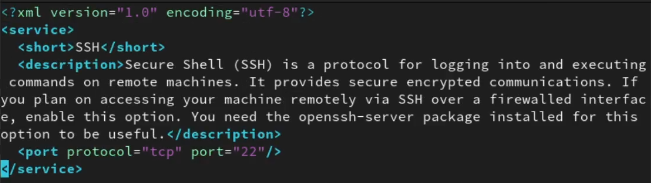
\includegraphics[width=\textwidth]{../images/image00.png}
    \captionof{figure}{Содержимое файла ssh.xml по умолчанию}
\end{frame}

\begin{frame}[containsverbatim]
\frametitle{Создание пользовательской службы firewalld}
\begin{minted}{bash}
<?xml version="1.0" encoding="utf-8"?>
<service>
  <short>SSH</short>
  <description>Modified SSH with port 2022.</description>
  <port protocol="tcp" port="2022"/>
</service>
\end{minted}
\end{frame}

\begin{frame}
\frametitle{Создание пользовательской службы firewalld}
    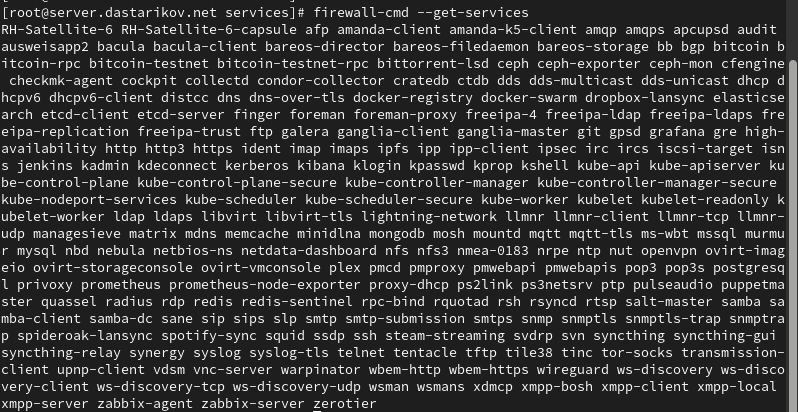
\includegraphics[width=\textwidth]{../images/image01.png}
    \captionof{figure}{Список доступных служб.}
\end{frame}

\begin{frame}
\frametitle{Создание пользовательской службы firewalld}
    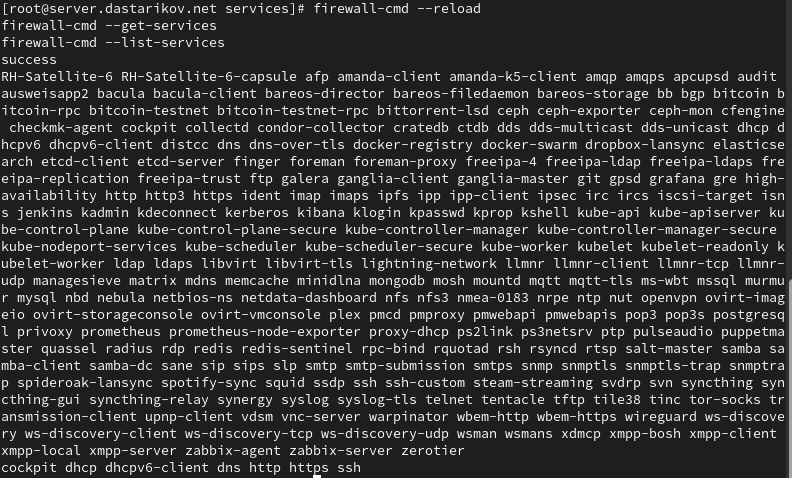
\includegraphics[width=\textwidth]{../images/image02.png}
    \captionof{figure}{Список доступных и активных служб после обновления.}
\end{frame}

\begin{frame}
\frametitle{Создание пользовательской службы firewalld}
    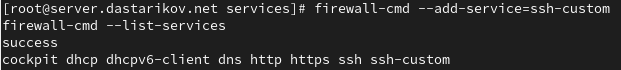
\includegraphics[width=\textwidth]{../images/image03.png}
    \captionof{figure}{Список активных служб после добавления ssh-custom.}
\end{frame}

\begin{frame}
\frametitle{Создание пользовательской службы firewalld}
    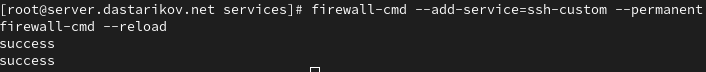
\includegraphics[width=\textwidth]{../images/image04.png}
    \captionof{figure}{Сохранение информации о состоянии и перезагрузка службы firewalld.}
\end{frame}


\begin{frame}
\frametitle{Перенаправление портов}
    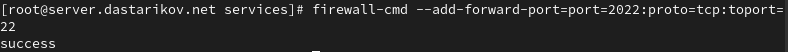
\includegraphics[width=\textwidth]{../images/image05.png}
    \captionof{figure}{Успешное добавление переадресации с порта 2022 на порт 22.}
\end{frame}

\begin{frame}
\frametitle{Перенаправление портов}
    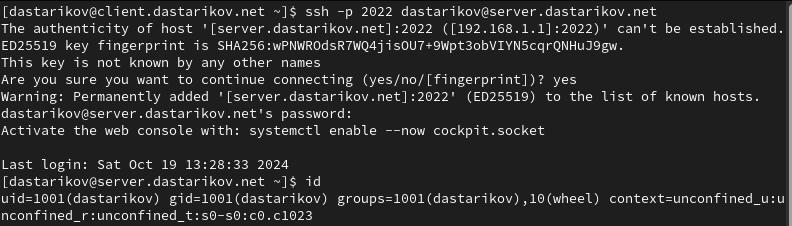
\includegraphics[width=\textwidth]{../images/image06.png}
    \captionof{figure}{Получение доступа по SSH на клиенте.}
\end{frame}


\begin{frame}
\frametitle{Настройка Port Forwarding и Masquerading}
    \centering
    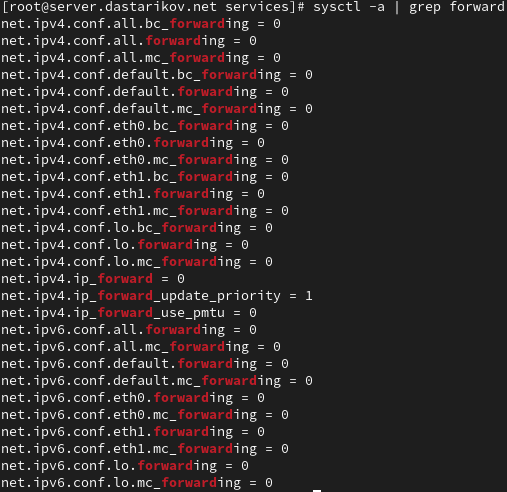
\includegraphics[width=0.7\textwidth]{../images/image07.png}
    \captionof{figure}{Список параметров, связанных с перенарпавлением пакетов.}
\end{frame}

\begin{frame}
\frametitle{Настройка Port Forwarding и Masquerading}
    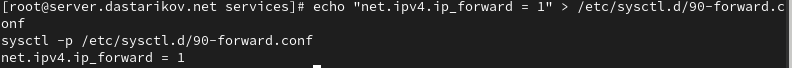
\includegraphics[width=\textwidth]{../images/image09.png}
    \captionof{figure}{Включение перенапрвления IPv4\-пакетов на сервере.}
\end{frame}

\begin{frame}
\frametitle{Настройка Port Forwarding и Masquerading}
    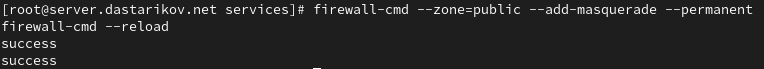
\includegraphics[width=\textwidth]{../images/image10.png}
    \captionof{figure}{Включение маскарадинга на сервере.}
\end{frame}

\begin{frame}
\frametitle{Настройка Port Forwarding и Masquerading}
    
\includegraphics[width=\textwidth]{../images/image11.png}
    \captionof{figure}{Проверка доступности Интернета на клиенте.}
\end{frame}

\begin{frame}
\frametitle{Внесение изменений в настройки внутреннего окружения виртуальной машины}
    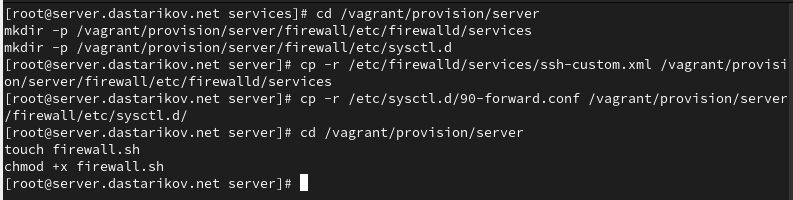
\includegraphics[width=\textwidth]{../images/image12.png}
    \captionof{figure}{Создание каталога с конфигурацией firewalld.}
\end{frame}

\begin{frame}[containsverbatim]
\frametitle{Внесение изменений в настройки внутреннего окружения виртуальной машины}
    \begin{minted}[breaklines=true]{bash}
#!/bin/shell
echo "Provisioning script \$0"
echo "Copy configuration files"
cp -R /vagrant/provision/server/firewall/etc/* /etc
echo "Configure masquerading"
firewall-cmd --add-service=ssh-custom --permanent
firewall-cmd --add-forward-port=port=2022:proto=tcp:toport=22 --permanent
firewall-cmd --zone=public --add-masquerade --permanent
firewall-cmd --reload
restorecon -vR /etc
    \end{minted}
\end{frame}

\begin{frame}
\frametitle{Внесение изменений в настройки внутреннего окружения виртуальной машины}
    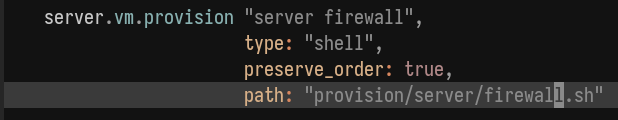
\includegraphics[width=\textwidth]{../images/image13.png}
    \captionof{figure}{Изменение Vagrantfile.}
\end{frame}


% \begin{frame}
% \frametitle{Две колонки}
% \begin{columns}
%     \column{0.5\textwidth}
%         \includegraphics[width=\textwidth]{../images/test.png}
%         \captionof{figure}{Изображение.}
%     \column{0.5\textwidth}
%         Текст на второй половине слайда.
% \end{columns}
% \end{frame}

\begin{frame}
\frametitle{Выводы}
\begin{itemize}
    \item В результате выполнения лабораторной работы продолжили изучать настройки межсетевого экрана в Linux, настроили переадресацию портов и Masquerading.
\end{itemize}
\end{frame}
\end{document}
